\lab{Applications}{Image Compression (SVD)}{SVD}

\objective{Explore the SVD as a method of image compression}

In this lab, we are going to explore how the SVD can be used to compress image data.  
Recall that the SVD is a decomposition of an $m \times n$ matrix $A$ of rank $r$ into the product $A = U \Sigma V^H$, where $U$ and $V$ are unitary matrices having dimensions $m \times m$ and $n \times n$, respectively, and $\Sigma$ is an $m \times n$ diagonal matrix.
\begin{equation*}
\Sigma = \mbox{diag}(\sigma_1,\sigma_2,\ldots,\sigma_r,0,\ldots,0)
\end{equation*}
where $\sigma_1 \geq \sigma_2 \geq \ldots \geq \sigma_r > 0$ are the singular values of $A$.
Upon closer inspection, we see that we can write
\begin{equation*}
U = \begin{pmatrix}U_1 & U_2\end{pmatrix}, \quad \Sigma =
\begin{pmatrix}\Sigma_r & 0\\0 & 0\end{pmatrix}, \quad V =
\begin{pmatrix}V_1 & V_2\end{pmatrix},
\end{equation*}
where $U_1$ and $V_1$ have dimensions $m\times r$ and $n\times r$ respectively and $\Sigma_r$ is the $r\times r$ diagonal matrix of (nonzero) singular values.
Multiplying this out yields the reduced form of the SVD
\begin{equation*}
A =
\begin{pmatrix}U_1 & U_2\end{pmatrix}
\begin{pmatrix}\Sigma_r & 0\\0 & 0\end{pmatrix}
\begin{pmatrix}V^H_1 \\ V^H_2\end{pmatrix} =
U_1 \Sigma_r V_1^H
\end{equation*}

\subsection*{Low rank data storage}
If the rank of a given matrix is significantly smaller than its dimensions, the reduced form of the SVD offers a way to store $A$ with less memory.
Without the SVD, an $m\times n$ matrix requires storing $m*n$ values.
By decomposing the original matrix into the SVD reduced form, $U_1$, $\Sigma_r$ and $V_1$ together require $(m*r)+r+(n*r)$ values.
Thus if $r$ is much smaller than both $m$ and $n$, we can obtain considerable efficiency.
For example, suppose $m=100$, $n=200$ and $r=20$. 
Then the original matrix would require storing $20,000$ values whereas the reduces form of the SVD only requires storing $6020$ values.

\subsection*{Low rank approximation}
The reduced form of the SVD also provides a way to approximate a
matrix with another one of lower rank.
This idea is used in many areas of applied mathematics including signal processing, statistics, semantic indexing (search engines), and control theory.
If we are given a matrix $A$ of rank $r$, we can find an approximate matrix $\widehat A$ of rank $s<r$ by taking the SVD of $A$ and setting all of its singular values after $\sigma_s$ to zero, that is,
\begin{equation*}
\Sigma_{\widehat A} = \sigma_1, \sigma_2, \ldots, \sigma_s,\sigma_{s+1}=0,\ldots,\sigma_r=0
\end{equation*}
and then multiplying the matrix back together again.
The more singular values we keep, the closer our approximation is to $A$.
The number of singular values we decide to preserve depends on how close of an approximation we need and what our size requirements are for $U_1$, $\Sigma_{\widehat A}$, and $V_1$.
Try plotting the the singular values.
We have plotted the singular values to the image below.
Matrix rank is on the x-axis and the eigenvalues are the y-axis.
Note that SVD orders the singular values from greatest to least.
The greatest eigenvalues contribute most to the image while the smallest eigenvalues hardly contribute anything to the final approximation.
By looking at the graph we can have a rough idea of how many singular values we need to preserve to have a good approximation of $A$.
The matrix rank of the image below is $670$.
However, as the plot shows, we could easily approximate the image using only the first half of the singular values.

%\begin{figure}
%\includegraphics[]{hubble_red.png}
%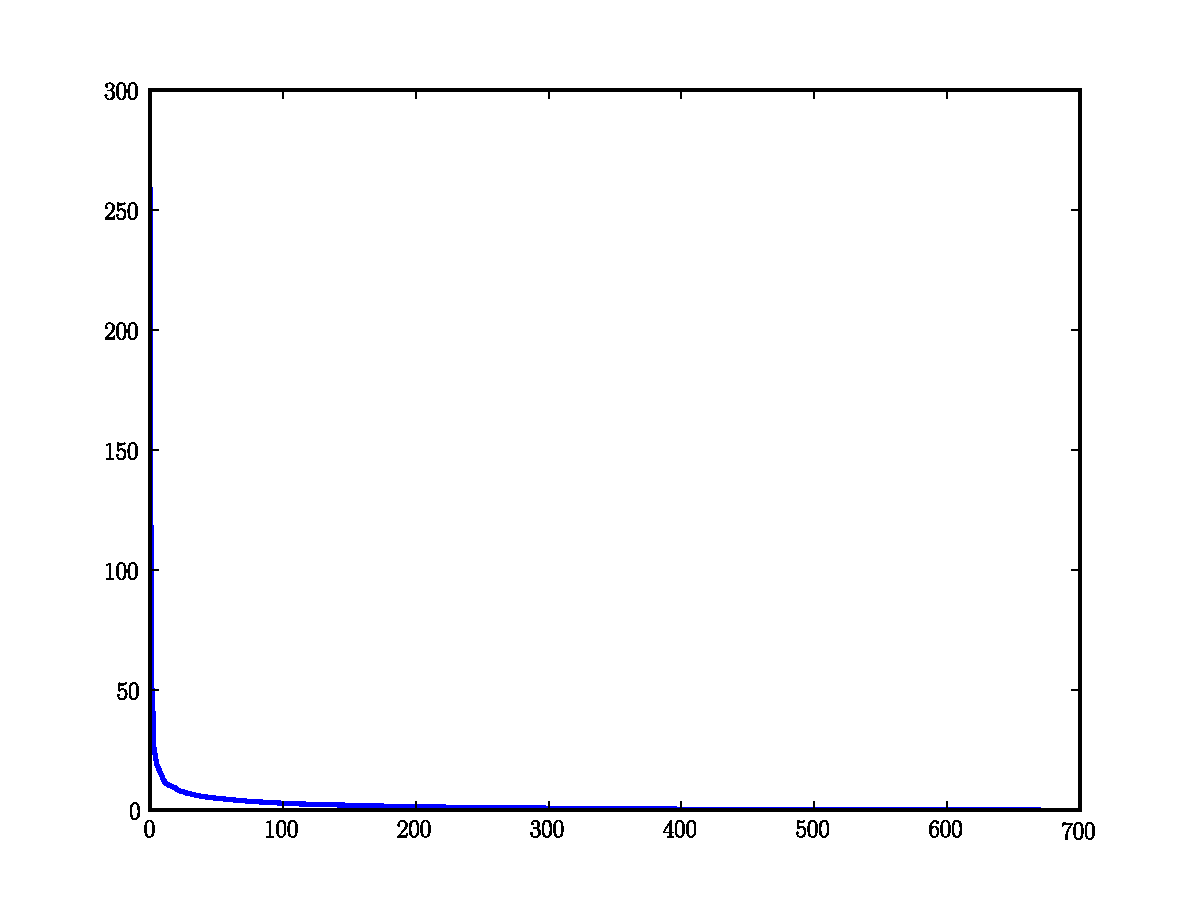
\includegraphics[scale=.4]{hubble_svals.pdf}
%\end{figure}

\begin{figure}
\begin{minipage}[b]{.4\linewidth}
\centering
\includegraphics[width=\textwidth]{hubble_red}
\end{minipage}
\hspace{0.5cm}
\begin{minipage}[b]{0.5\linewidth}
\centering
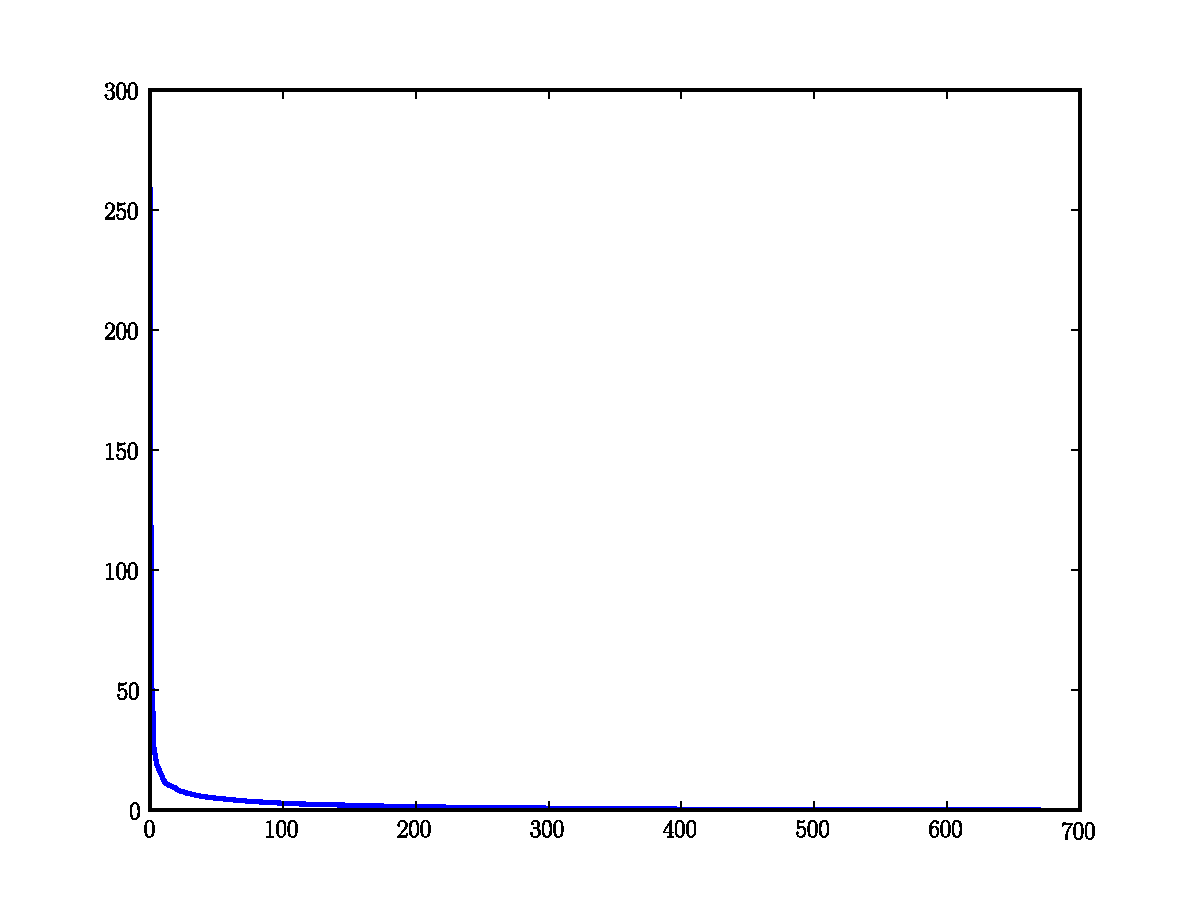
\includegraphics[width=\textwidth]{hubble_svals}
\end{minipage}
\caption{An image and its SVD.}
\end{figure}

\begin{lstlisting}
: import numpy as np
: from scipy.linalg import svd, norm
: A = np.array([[1,1,3,4], [5,4,3,7], [9,10,10,12], [13,14,15,16], [17,18,19,20]])
: U,s,Vt = svd(A)
: S = np.diag(s)
: Ahat = U[:,0:3].dot(S[0:3,0:3]).dot(Vt[0:3,:])
: norm(A-Ahat)
\end{lstlisting}
Note that $\widehat A$ is ``close'' to the original matrix $A$, but that its rank is 3 instead of 4.

\subsection*{Application to Imaging}
Enter the following into IPython (note that any image you might have will work):
\begin{lstlisting}
: import matplotlib.pyplot as plt
: X = plt.imread('fingerprint.png')[:,:,0].astype(float)
: X.nbytes      #number of bytes needed to store X
: plt.imshow(X)
: plt.show()
\end{lstlisting}
Computing the SVD of your image is simple.
Remember to make the singular values a diagonal matrix before multiplying.
\begin{lstlisting}
: U,s,Vt = svd(X)
: S = sp.diag(s)
\end{lstlisting}
In the next code block, $n$ represents the desired rank of the output.
\begin{lstlisting}
: n = 50
: u1, s1, vt1 = U[:,0:n], S[0:n,0:n], Vt[0:n,:]
: Xhat = u1.dot(s1).dot(vt1)
: (u1.nbytes + np.diag(s1).nbytes + vt1.nbytes) - X.nbytes   #should be negative
: plt.imshow(Xhat)
: plt.show()
\end{lstlisting}

\begin{problem}
Sometimes there is not enough available bandwidth to transmit a full resolution photograph.
You aim to reduce the amount of data that needs to be transmitted from a remote location such that loss of image detail is minimal, but the amount of data that needs to be sent has reduced as much as possible.
In other words, find the minimum rank needed to accurately represent a variety of images.
Record your results and comment on them.
\end{problem}
